\documentclass[border = 1.5cm]{standalone}

%%%% packages
\usepackage{tikz}
\usepackage{tikzpeople}
\usetikzlibrary{trees,
                arrows,
                shapes.geometric,
                positioning,
                fit}
%% document
\begin{document}
%% styles
\tikzset{
    font = {\fontsize{13pt}{12}\sffamily},
	element/.style = {rectangle, rounded corners, minimum width = 4cm, minimum height = 3cm, text centered, draw = black},
    filter/.style = {rectangle, rounded corners, align = center, anchor = west, yshift = -1cm},
    frame/.style = {draw, rectangle, rounded corners, dashed, blue, line width = 1pt, inner sep = 4mm}, %, dash pattern=on 1pt off 4pt on 6pt off 4pt},
    arrow1/.style = {->, thick},
    arrow2/.style = {->, line width = 3pt}
}
%% layers
\pgfdeclarelayer{bg1}
\pgfsetlayers{bg1, main}
%% tikzpicture
\begin{tikzpicture}[
	grow via three points = {one child at (0.5,-1) and
		                     two children at (0.5,-1) and
		                     (0.5,-1.7)},
	edge from parent path = {(\tikzparentnode.south) |- (\tikzchildnode.west)},
	inner sep = 0cm, outer sep = 0cm
	]
%% person
\node (person) [bob, minimum size = 2cm] at (0,0) {};
%% app
\node (stx-app-screenshot) [right of = person, xshift = 5cm, yshift = 3cm] {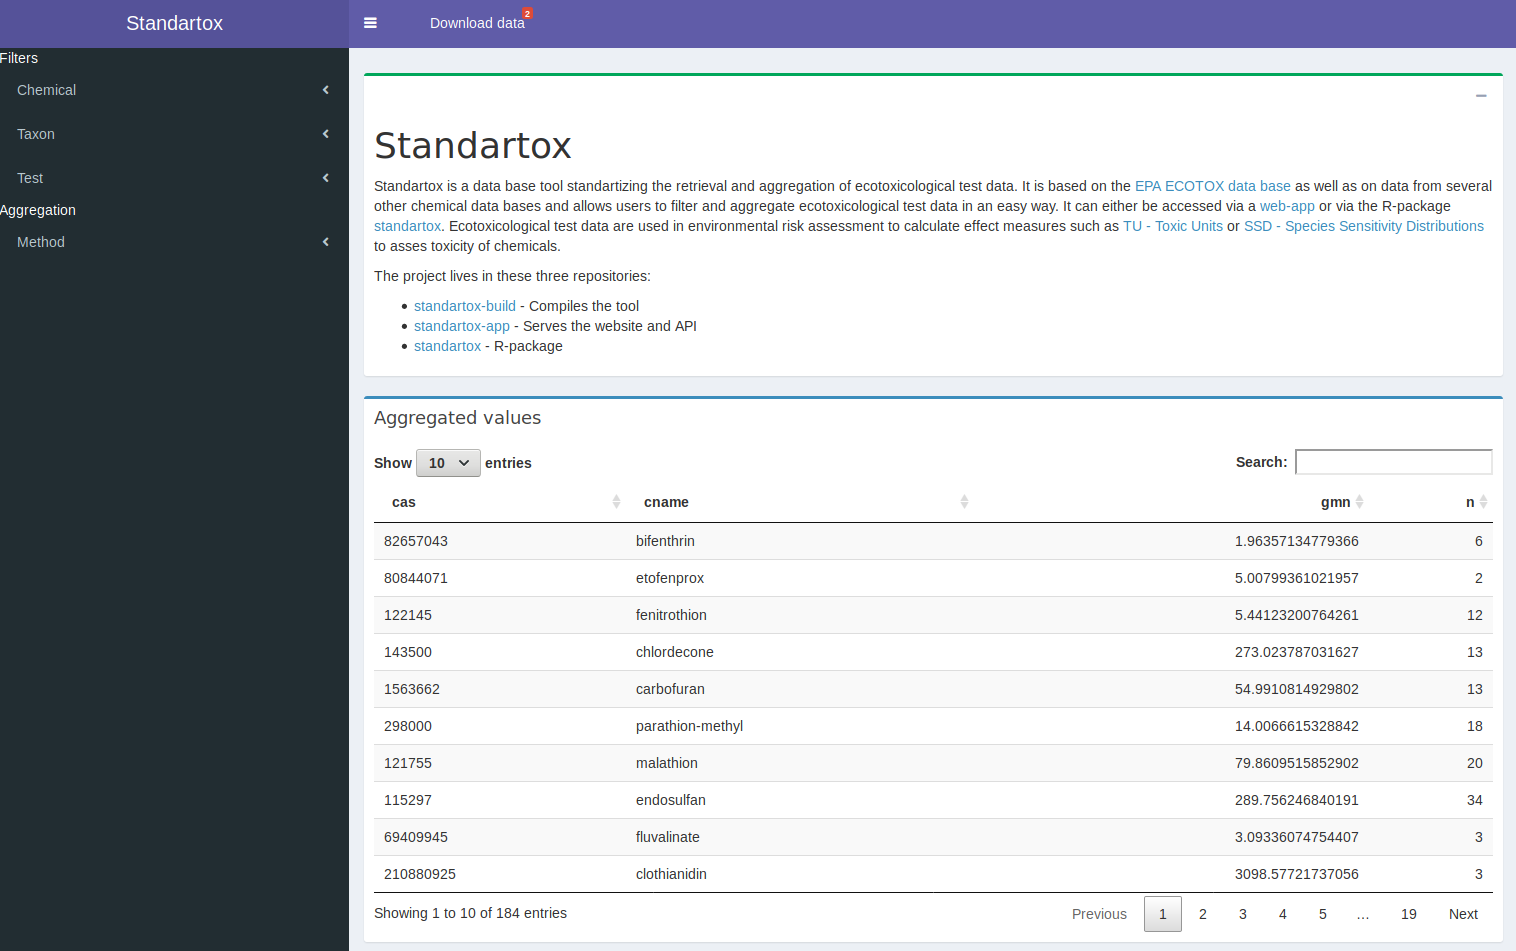
\includegraphics[width=.35\textwidth]{article/figures/screenshot_standartox_app.png}};
\node (stx-rpackage-screenshot) [right of = person, xshift = 5cm, yshift = -3cm] {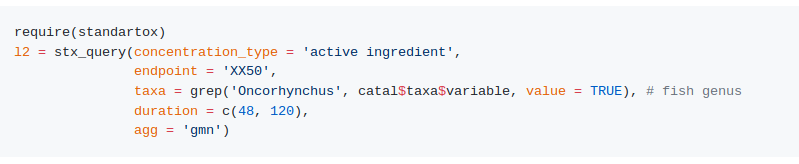
\includegraphics[width=.35\textwidth]{article/figures/screenshot_standartox_rpackage.png}};
%% elements
\node (epa-ecotox) [element, right of = person, xshift = 13cm, yshift = 5.5cm, fill = gray] {EPA ECOTOX};
\node (filtered) [element, below of = epa-ecotox, yshift = -3cm] {Filtered Data}
    child {node [filter] {CAS}}
    child {node [filter] {Concentration type}}
    child {node [filter] {Chemical class}}
    child {node [filter] {Taxa}}
    child {node [filter] {Habitat}}
    child {node [filter] {Region}}
    child {node [filter] {Duration}}
    child {node [filter] {Effect}}
    child {node [filter] {Endpoint}}
    child {node (filter-last) [filter] {Version}}
    ;
\node (aggregated) [element, right of = filtered, xshift = 7cm] {Aggregated Data};
\node (meta) [element, below of = aggregated, yshift = -5cm] {Meta Information};
%% frames
\node (frame-stx) [frame, fit = (epa-ecotox) (filter-last) (meta) ] {};
\node (frame-stx-text) [above, blue, inner sep = 2mm] at (frame-stx.north) {Standartox data set};
\node (frame-app) [frame, fit = (stx-app-screenshot)] {};
\node (frame-app-text) [above, blue, inner sep = 2mm] at (frame-app.north) {APP};
\node (frame-api) [frame, fit = (stx-rpackage-screenshot)] {};
\node (frame-api-text) [above, blue, inner sep = 2mm] at (frame-api.north) {API};
\node (frame-rpackage) [frame, fit = (frame-api) (frame-api-text)] {};
\node (frame-rpackage-text) [above, blue, inner sep = 2mm] at (frame-rpackage.north) {R package};
%% arrows
\draw [arrow1] (filtered.east) -- (aggregated.west);
\draw [arrow1] (epa-ecotox.south) -- (filtered.north);
\begin{pgfonlayer}{bg1}
    \draw [arrow2] (person.north east) to[bend left = 10] (frame-stx.150);
    \draw [arrow2] (person.south east) to[bend right = 10] (frame-stx.210);
\end{pgfonlayer}
\end{tikzpicture}
\end{document}